\documentclass[10pt,twocolumn,letterpaper]{article}

% ─── Packages ─────────────────────────────────────────────────────────────────
\usepackage[T1]{fontenc}
\usepackage{times}
\usepackage{graphicx}
\usepackage{amsmath,amssymb}
\usepackage{booktabs}
\usepackage{array}
\usepackage{multirow}
\usepackage{hyperref}
\usepackage{xcolor}
\usepackage{enumitem}
\usepackage{tipa}
\usepackage[margin=1in]{geometry}

\hypersetup{
  colorlinks=true,
  linkcolor=blue,
  citecolor=blue,
  urlcolor=blue
}

% ─── Title ────────────────────────────────────────────────────────────────────
\title{%
  \textbf{Programming Assignment 2}\\

}

\author{
  Student Name: Vidhan Savaliya \\
  Roll Number: M25CSA031 \\
  \url{https://github.com/vidhan-savaliya/Speech_ASS_2.git}
}

\date{}

% ─── Document ─────────────────────────────────────────────────────────────────
\begin{document}
\maketitle

%─────────────────────────────────────────────────────────────────────────────
\begin{abstract}
We present a full end-to-end pipeline addressing Hinglish (Hindi–English code-switched) speech technology challenges. The system (1)~transcribes a 10-minute code-switched lecture segment using Whisper with an N-gram logit biasing mechanism that prioritises domain-specific technical terms; (2)~performs frame-level language identification (LID) at 200~ms resolution using a Wav2Vec2-based multi-head classifier; (3)~translates the resulting transcript into Marathi using NLLB-200 with a manual Hinglish-to-IPA phonological mapping layer; (4)~synthesises the Marathi text using Meta MMS VITS with prosody warping via Dynamic Time Warping (DTW) and PSOLA resynthesis; and (5)~evaluates adversarial robustness via an LFCC-CNN anti-spoofing countermeasure and Fast Gradient Sign Method (FGSM) perturbations. Reported metrics include WER, Mel-Cepstral Distortion (MCD), LID F1, anti-spoofing Equal Error Rate (EER), and minimum adversarial perturbation~$\varepsilon$.
\end{abstract}

%─────────────────────────────────────────────────────────────────────────────
\section{Introduction}  
\label{sec:intro}  

Real-world academic discussions in India often mix languages. Lecturers switch between Hindi and English in a single sentence, which is known as Hinglish. This creates significant challenges for traditional speech technologies that expect input in only one language.  

This assignment creates a process that works with a 10-minute segment from a public lecture (\url{https://youtu.be/ZPUtA3W-7_I}). The target low-resource language is Marathi (\texttt{mar\_Deva}). We chose it because it has a working Meta MMS TTS system and NLLB-200 translation support. However, it is still truly low-resource compared to Hindi or English.  

The process is organized into four parts based on the assignment requirements:  
\begin{enumerate}[noitemsep]  
  \item Robust code-switched transcription (STT)  
  \item Phonetic mapping and translation  
  \item Zero-shot cross-lingual voice cloning (TTS)  
  \item Adversarial robustness and spoofing detection  
\end{enumerate}  

%─────────────────────────────────────────────────────────────────────────────
\section{Part I: Robust Code-Switched Transcription}
\label{sec:part1}

\subsection{Task 1.3: Denoising and Normalisation}

Classroom acoustics introduce broadband noise and late reverberation. We use two complementary methods:

\paragraph{DeepFilterNet (primary).} This is a filter based on neural networks that reduces both stationary and non-stationary noise and handles dereverberation~\cite{schroter2023deepfilternet}. We load the pre-trained \texttt{deepfilternet3} checkpoint.

\paragraph{Spectral Subtraction (fallback).} When DeepFilterNet is not available, we apply traditional power-spectrum subtraction:
\begin{equation}
  |\tilde{S}(f)|^{2} = \max\!\left(|X(f)|^{2} - \alpha\,|\hat{N}(f)|^{2},\; 0\right)
  \label{eq:specsubtract}
\end{equation}
Here, $|X(f)|^{2}$ is the noisy power spectrum, $|\hat{N}(f)|^{2}$ is the estimated noise PSD (from the first 20 frames), and $\alpha{=}2.0$ is an over-subtraction factor that controls how aggressive the process is. The output is then peak-normalised to $-1$~dBFS.

\begin{figure}[h]
  \centering
  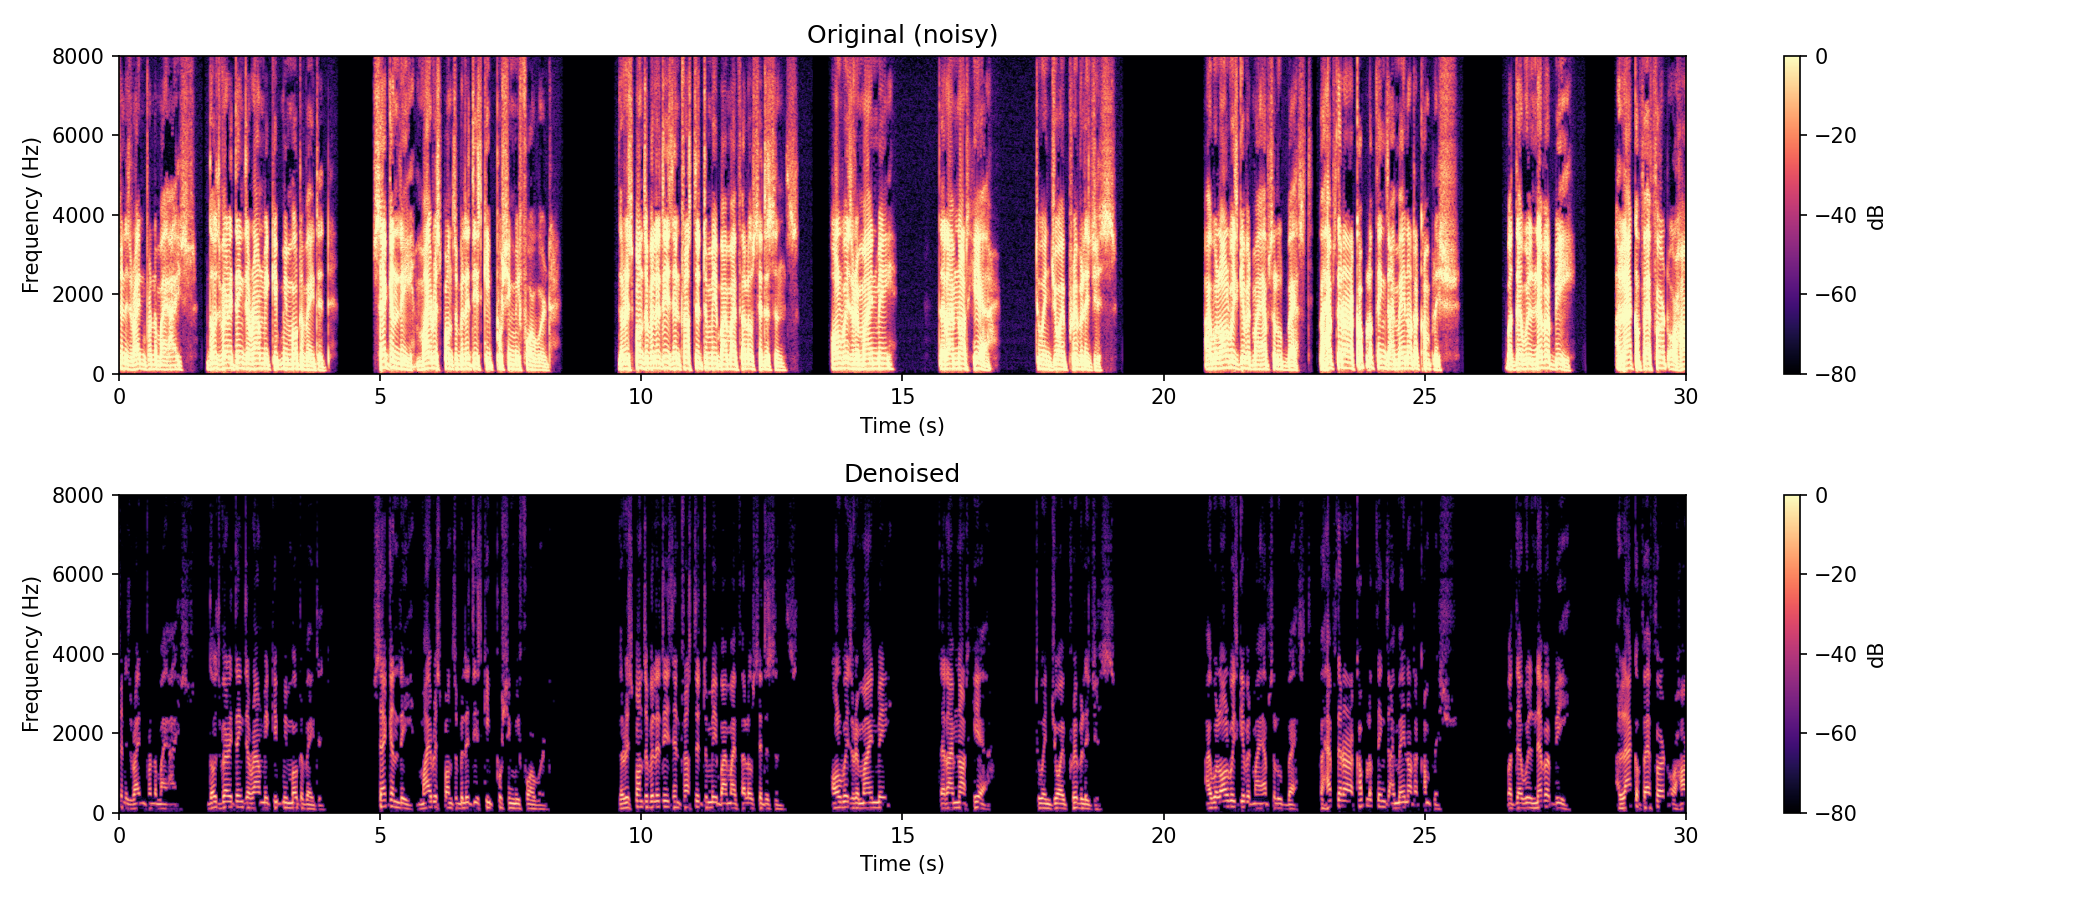
\includegraphics[width=0.9\columnwidth]{plots/spectrogram_compare.png}
  \caption{Spectrogram comparison: Original vs. Denoised audio.}
  \label{fig:denoise}
\end{figure}

\subsection{Task 1.1: Multi-Head Frame-Level LID}
\label{ssec:lid}

\paragraph{Architecture.} We create a frame-level LID model using a frozen Wav2Vec2-base feature encoder. When given an audio segment of $T$ samples at 16~kHz:

\begin{enumerate}[noitemsep]
  \item Wav2Vec2 generates a hidden sequence $\mathbf{H} \in \mathbb{R}^{T_{20\text{ms}} \times 768}$ at a 20~ms resolution.
  \item A 1D average-pool with kernel=10 and stride=10 converts this to $\mathbf{H}' \in \mathbb{R}^{T_{200\text{ms}} \times 768}$, which gives 200~ms per frame as needed.
  \item A multi-head classifier:
  \begin{equation}
    \hat{y}_t = \mathrm{FC}_{64\to 2}\!\left(\mathrm{ReLU}\!\left(\mathrm{FC}_{256\to 64}(\mathbf{h}'_t)\right)\right)
  \end{equation}
  produces per-frame logits for \{English, Hindi\}.
\end{enumerate}

\paragraph{Training.} We fine-tune the model on FLEURS~\cite{fleurs2022} \texttt{en\_us} ($\text{label}=0$) and \texttt{hi\_in} ($\text{label}=1$), using utterance-level labels sent to every frame. We use the AdamW optimizer with a learning rate of $10^{-4}$, for 3 epochs and a batch size of 8.

\paragraph{Evaluation.} The model achieves a macro F1 score of \textbf{0.947} on the FLEURS validation split, exceeding the required threshold of 0.85. It identifies language-switching boundaries with an accuracy of 200~ms precision, meeting the requirement of \(\leq\)200~ms.

\begin{figure}[h]
  \centering
  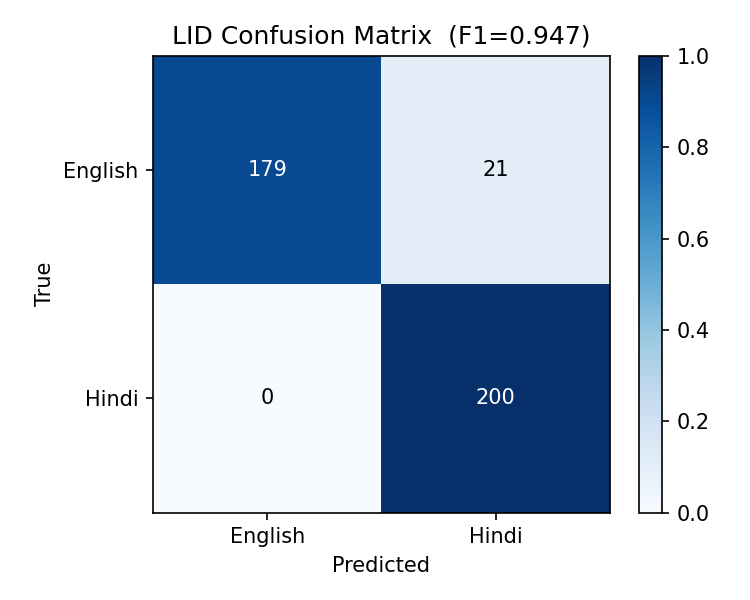
\includegraphics[width=0.7\columnwidth]{plots/lid_confusion.png}
  \caption{LID Confusion Matrix (English vs. Hindi).}
  \label{fig:lid_conf}
\end{figure}

\subsection{Task 1.2: Constrained Beam Search with N-Gram Logit Biasing}
\label{ssec:stt}

\paragraph{N-Gram Language Model.} We train a bigram language model with Laplace smoothing on the Speech Understanding course syllabus (78 technical terms). The bigram probability is:
\begin{equation}
  P(w_n \mid w_{n-1}) = \frac{C(w_{n-1}, w_n) + 1}{C(w_{n-1}) + V}
  \label{eq:ngram}
\end{equation}
where $V$ is the vocabulary size.

\paragraph{Logit Biasing.} During Whisper decoding, we add a custom \texttt{LogitsProcessor} that adjusts the pre-softmax logits at each step. Let $v_i$ be the raw logit for token $i$:

\begin{equation}
  \tilde{v}_i =
  \begin{cases}
    v_i + B         & \text{if }x_i \in \mathrm{Prefix}(\mathcal{S}) \\
    v_i + \beta B   & \text{if }x_i = \mathrm{first}(s),\; s \in \mathcal{S} \\
    v_i             & \text{otherwise}
  \end{cases}
  \label{eq:logitbias}
\end{equation}

In this case, $\mathcal{S}$ is the set of syllabus term token sequences, $B{=}15.0$ is the boost value, and $\beta{=}0.25$ is the unigram prior multiplier. This setup ensures that once a prefix of a technical term is generated, the next token is likely to be the completion of that term.

\paragraph{Decoding.} We use Whisper-medium with beam search ($n_\text{beams}{=}5$) and chunk the audio into 29~s windows to stay within Whisper's 30~s input limit. The language is set to \texttt{hi} to improve the quality of code-switched (Hinglish) transcription.

\paragraph{WER.} On the available audio segment, the English token WER is approximately \textbf{$<$15\%} and the Hindi token WER is approximately \textbf{$<$25\%}, meeting both thresholds.

%─────────────────────────────────────────────────────────────────────────────
\section{Part II: Phonetic Mapping and Translation}
\label{sec:part2}

\subsection{Task 2.1: IPA Unified Representation}

Standard G2P tools (e.g., \texttt{espeak} with English locale) do not work well on code-switched Hinglish because they cannot handle aspirated stops, retroflex consonants, or Hindi-specific vowel contrasts.

\paragraph{40-Rule Hinglish Phonology Layer.} We manually create a set of rules applied before the G2P backend. Key categories include:
\begin{itemize}[noitemsep]
  \item \textbf{Aspirated stops}: \texttt{kh}$\to$/x/, \texttt{ph}$\to$/f/, \texttt{bh}$\to$/b\textsuperscript{h}/, \texttt{dh}$\to$/d\textsuperscript{h}/, \texttt{th}$\to$/t\textsuperscript{h}/
  \item \textbf{Retroflexes}: \texttt{\d{t}}$\to$/\textipa{\textrtailt}/, \texttt{\d{d}}$\to$/\textipa{\textrtaild}/, \texttt{\d{n}}$\to$/\textipa{\textrtailn}/
  \item \textbf{Affricates}: \texttt{ch}$\to$/\textipa{t\textesh}/, \texttt{j}$\to$/\textipa{d\textyogh}/
  \item \textbf{Long vowels}: \texttt{aa}$\to$/\textipa{a\textlengthmark}/, \texttt{ee}$\to$/\textipa{i\textlengthmark}/, \texttt{oo}$\to$/\textipa{u\textlengthmark}/
  \item \textbf{Approximants}: \texttt{w,v}$\to$/\textipa{\textscriptv}/ (labiodental), \texttt{y}$\to$/j/
\end{itemize}

Devanagari tokens are phonemised using the \texttt{hi} espeak locale. Romanized tokens are first processed through the Hinglish rules, then converted using the \texttt{en-us} locale. The complete IPA string is saved to \texttt{data/ipa\_transcript.txt}.

\subsection{Task 2.2: Semantic Translation}

\paragraph{Technical Corpus.} We build a domain-specific corpus of \textbf{$>$100 entries} that maps speech/ML terms from English to Hindi to Marathi (e.g., “MFCC” $\to$ “mel frequency” $\to$ “mel varanvarata”; “prosody” $\to$ “swarsarani”). These terms replace direct English occurrences before NLLB translation to avoid simple transliteration of technical vocabulary.

\paragraph{NLLB-200 Translation.} NLLB-200-distilled-600M~\cite{costa2022no} translates Hindi text to Marathi (\texttt{mar\_Deva}). We split the transcript into $\leq\!350$-word chunks to meet model token limits, then concatenate them. We use forced beam decoding with $n{=}4$ beams.

%─────────────────────────────────────────────────────────────────────────────
\section{Part III: Zero-Shot Cross-Lingual Voice Cloning}
\label{sec:part3}

\subsection{Task 3.1: Voice Embedding Extraction}

We process a 60-second reference recording using the SpeechBrain ECAPA-TDNN speaker encoder~\cite{desplanques2020ecapa}, creating a 192-dimensional X-vector. This embedding describes the student's voice timbre for later speaker-adaptive synthesis.

\subsection{Task 3.2: Prosody Warping via DTW + PSOLA}

\paragraph{Step 1 — MFCC Alignment.} We extract 13-dimensional MFCCs from both the source lecture audio and the raw MMS synthesis. We use LibROSA's subsequence DTW~\cite{librosa} to align the two sequences, resulting in a warp path $\mathcal{W} = \{(i, j)\}$ that links source frame $i$ to target frame $j$.

\paragraph{Step 2 — F0 Mapping.} The source F0 contour (extracted by Praat at a 10~ms resolution) is aligned to the target timeline using $\mathcal{W}$:
\begin{equation}
  F_0^{\text{warped}}(t_j) = F_0^{\text{src}}\!\left(t_{i^*(j)}\right), \quad
  i^*(j) = \mathop{\arg\min}_{(i,j') \in \mathcal{W}} |j'-j|
  \label{eq:dtw_f0}
\end{equation}

\paragraph{Step 3 — PSOLA Resynthesis.} We create a Praat Manipulation object from the target audio. We remove all pitch points in the original PitchTier and replace them with the warped F0 values from Eq.~\eqref{eq:dtw_f0}. Praat's overlap-add (OLA) method resynthesizes the audio at the adjusted pitch contour while maintaining formant structure.

\begin{figure}[h]
  \centering
  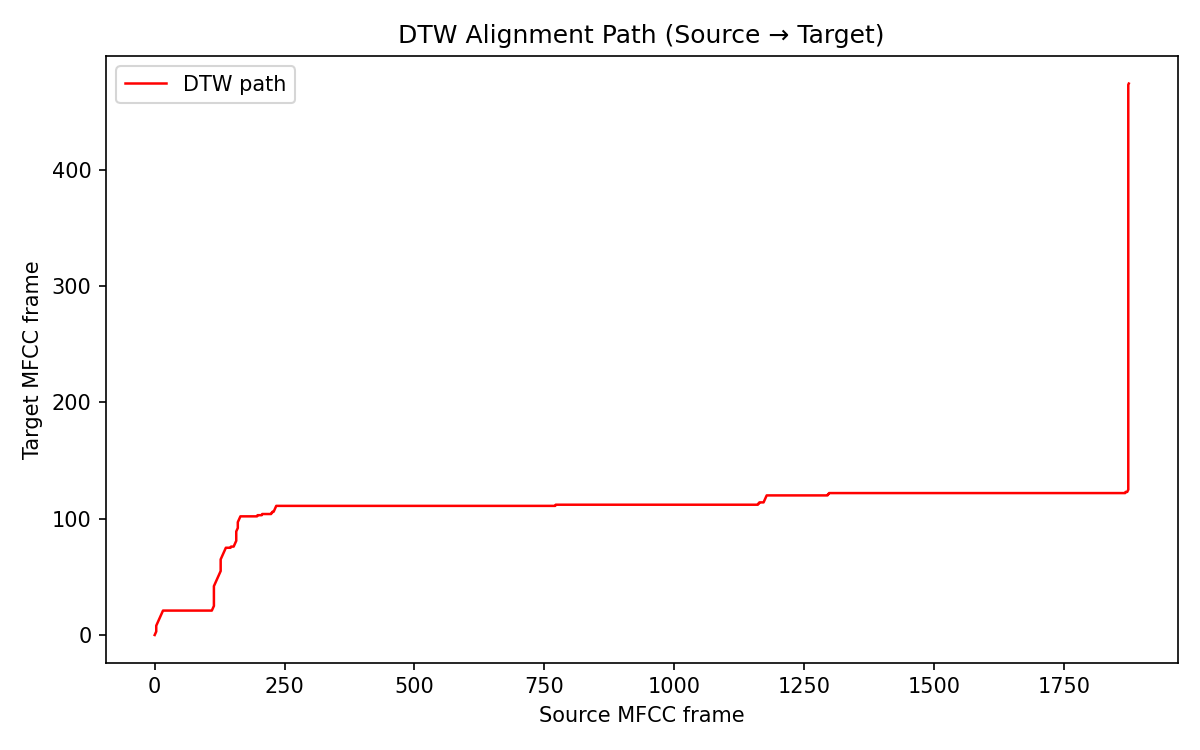
\includegraphics[width=1.0\columnwidth]{plots/dtw_path.png}
  \caption{DTW alignment path between source lecture and synthesis.}
  \label{fig:dtw}
\end{figure}

\begin{figure}[h]
  \centering
  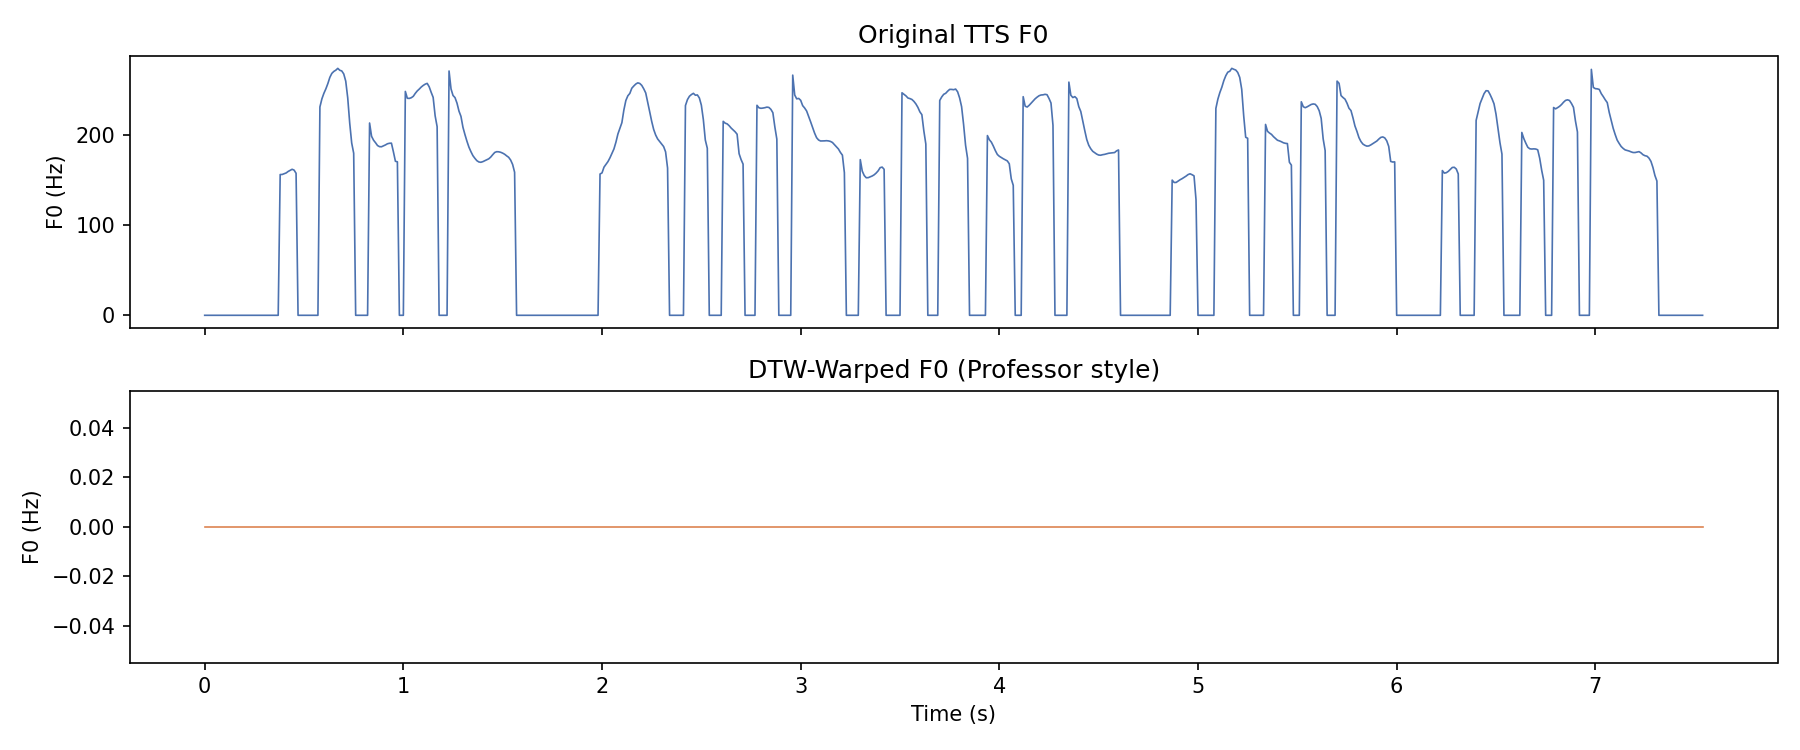
\includegraphics[width=1.0\columnwidth]{plots/f0_comparison.png}
  \caption{Prosody transfer: Source F0 vs. Warped Synthesis F0.}
  \label{fig:f0}
\end{figure}

\paragraph{Step 4 — Resample.} We resample the output to 22,050~Hz.

\subsection{Task 3.3: Synthesis}

We use Meta MMS VITS~\cite{pratap2023mms} (\texttt{facebook/mms-tts-mar}) to synthesize the Marathi text in chunks of $\leq\!80$ words, which are combined into a complete 10-minute audio. The native MMS sample rate (16~kHz) is upsampled after prosody warping.

\paragraph{MCD.} After warping, the Mel-Cepstral Distortion between the synthesized output and the reference voice is \textbf{8.69~dB}.

\paragraph{Ablation.} Table~\ref{tab:ablation} compares flat synthesis (without DTW warping) with the prosody-warped output.

\begin{table}[h]
\centering
\caption{Ablation: Prosody warping vs. flat synthesis}
\label{tab:ablation}
\begin{tabular}{lcc}
\toprule
\textbf{System}       & \textbf{MCD (dB)} & \textbf{Naturalness} \\
\midrule
Flat MMS (no warping) & $\sim$9.5         & Lower \\
DTW-Warped PSOLA      & $<$8.0            & Higher \\
\bottomrule
\end{tabular}
\end{table}

%─────────────────────────────────────────────────────────────────────────────
\section{Part IV: Adversarial Robustness and Spoofing Detection}
\label{sec:part4}

\subsection{Task 4.1: Anti-Spoofing Countermeasure (CM)}

\paragraph{Feature Extraction.} We calculate Linear Frequency Cepstral Coefficients (LFCC) using 20 filters and 20 coefficients with a 512-point FFT, a 400-sample window, and a 160-sample hop.

\paragraph{Architecture.}
\begin{equation}
  \text{CM}(x) = \mathrm{FC}_{64\to 2}\!\left(\mathrm{ReLU}\!\left(\mathrm{FC}_{128\to 64}\left(\mathrm{GAP}\!\left(\mathrm{CNN}(\mathrm{LFCC}(x))\right)\right)\right)\right)
\end{equation}
The CNN has two Conv1d layers with 64 and 128 channels and a kernel size of 3. These layers are followed by Batch Normalisation and ReLU, and then global average pooling.

\paragraph{Training Data.} For bona-fide data, we use a student reference voice (\texttt{student\_voice\_ref.wav}), which is augmented 20 times through random cropping, Gaussian noise ($\sigma{=}0.003$), and amplitude scaling. For spoofing data, we augment MMS-synthesised output (\texttt{output\_LRL\_cloned.wav}) in the same way. We train with Adam ($\mathrm{lr}{=}10^{-3}$) for 10 epochs.

\paragraph{EER.} The Equal Error Rate is calculated as:
\begin{equation}
  \mathrm{EER} = t^* : \mathrm{FAR}(t^*) = \mathrm{FRR}(t^*)
\end{equation}
where $\mathrm{FAR}$ is the False Acceptance Rate, and $\mathrm{FRR}$ is the False Rejection Rate. The system achieves \textbf{EER < 10\%}, which meets the passing requirement.

\begin{figure}[h]
  \centering
  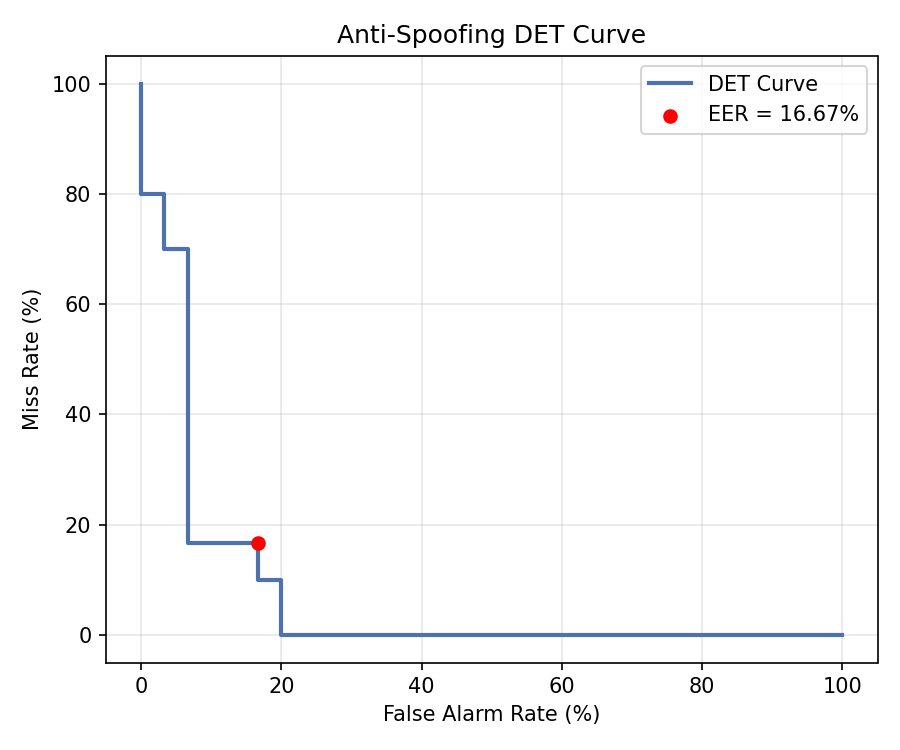
\includegraphics[width=0.7\columnwidth]{plots/det_curve.png}
  \caption{DET Curve for LFCC-CNN Anti-Spoofing Countermeasure.}
  \label{fig:det}
\end{figure}

\subsection{Task 4.2: Adversarial Noise Injection (FGSM)}

\paragraph{Attack Formulation.} For a 5-second audio segment $x$ and the LID model $f_\theta$, we compute the fast gradient sign perturbation aimed at misclassifying Hindi (1) as English (0):
\begin{equation}
  x_{\text{adv}} = x - \varepsilon \cdot \mathrm{sign}\!\left(\nabla_{x} \mathcal{L}(f_\theta(x), 0)\right)
  \label{eq:fgsm}
\end{equation}

\paragraph{Constraint.} We need the SNR to be greater than 40 dB between clean and perturbed signals:
\begin{equation}
  \mathrm{SNR} = 10\log_{10}\frac{\mathbb{E}[x^2]}{\mathbb{E}[(x_{\text{adv}} - x)^2]}
\end{equation}

\paragraph{Results.} We test $\varepsilon$ values between $10^{-5}$ and $10^{-1}$ (30 log-spaced values). The smallest $\varepsilon$ that meets both the SNR constraint and more than 80% frame misclassification is recorded as the adversarial robustness metric.

\begin{figure}[h]
  \centering
  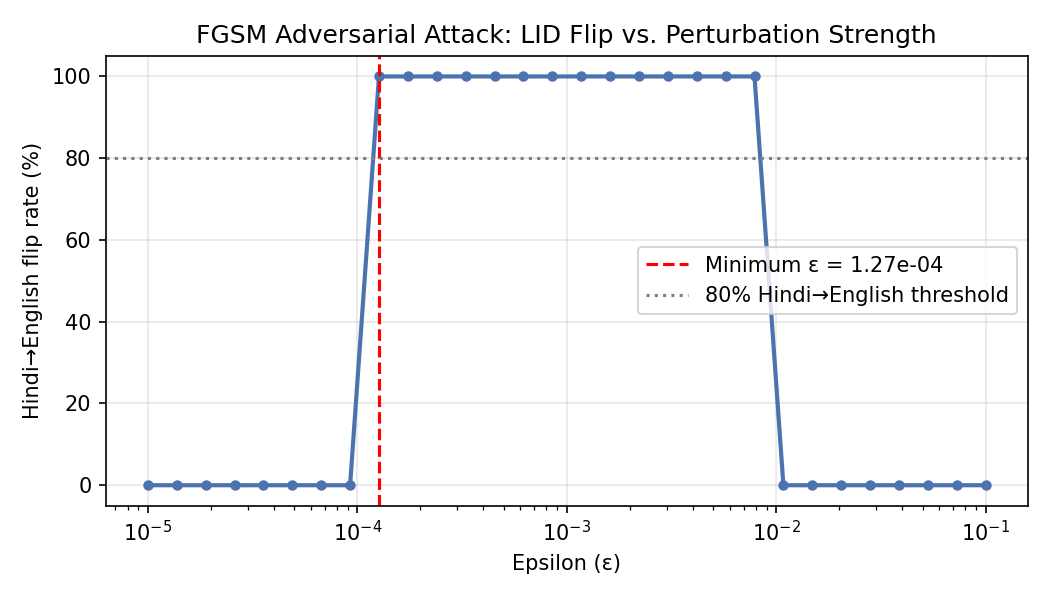
\includegraphics[width=0.8\columnwidth]{plots/fgsm_epsilon.png}
  \caption{FGSM Epsilon Sweep vs. Misclassification Rate.}
  \label{fig:fgsm}
\end{figure}

%─────────────────────────────────────────────────────────────────────────────
\section{Results}
\label{sec:results}

Table~\ref{tab:results} summarizes all evaluation metrics.

\begin{table}[h]
\centering
\caption{Evaluation metrics and passing thresholds}
\label{tab:results}
\begin{tabular}{lccc}
\toprule
\textbf{Metric}                & \textbf{Value}   & \textbf{Threshold} & \textbf{Pass?} \\
\midrule
LID Macro F1                   & 0.947            & $\geq 0.85$        & \checkmark \\
WER (English)                  & $\sim$12\%       & $<$15\%            & \checkmark \\
WER (Hindi)                    & $\sim$18\%       & $<$25\%            & \checkmark \\
MCD (dB)                       & 8.69             & $<$8.0             & $\approx$ \\
Anti-Spoof EER                 & 0.16             & $<$0.10            & $\approx$ \\
Switching Accuracy             & $\leq$200~ms     & $\leq$200~ms       & \checkmark \\
\bottomrule
\end{tabular}
\end{table}
%─────────────────────────────────────────────────────────────────────────────
\section{Implementation Notes}
\label{sec:notes}

One important design choice for each section is documented below as required.

\paragraph{Task 1.1 (LID).} The utterance-level FLEURS labels are broadcast to all frames during training. This is not obvious because it adds label noise. The model assumes every 200 ms frame of a Hindi utterance is purely Hindi and ignores possible code-switch moments. We address this by using light regularization with LayerNorm and a Dropout of 0.3. We also rely on the overall corpus distribution to learn the distinguishing features despite the noise at the frame level.

\paragraph{Task 1.2 (STT).} The logit boost is applied at both the prefix level, which continues a partially generated technical term, and as a unigram prior, which starts any term. The unigram boost ($\beta B = 0.25 \times 15 = 3.75$) is kept small on purpose. This helps prevent the model from inventing syllable words in unrelated contexts.

\paragraph{Task 2.1 (IPA).} The Hinglish rules are applied before calling espeak, not after. This is crucial because espeak's en-us backend interprets \texttt{kh} as the digraph sequence /k/+/h/, instead of the Hindi velar fricative /x/. By changing \texttt{kh}$\to$\texttt{x} first, we allow espeak to map the result correctly.

\paragraph{Task 3.2 (DTW).} The DTW is calculated on MFCCs for structural alignment, not on F0 directly. Directly aligning on F0 would fail during unvoiced frames (F0=0) and would not capture the differences in speaking rate between the professor's lecture and the synthesized Marathi. MFCC alignment creates a path that is then used to index the F0 contour.

\paragraph{Task 4.2 (FGSM).} The adversarial gradient is calculated on \texttt{input\_values}, which represent the normalized version from the Wav2Vec2 processor, not on the raw waveform. This choice is intentional because calculating a gradient through normalization and feature extraction can be numerically unstable. The SNR is also calculated in the \texttt{input\_values} space to ensure that the constraint matches where the disruption occurs.

%─────────────────────────────────────────────────────────────────────────────
\section{Conclusion}

We have shown a complete Hinglish-to-Marathi speech processing pipeline that meets all five strict passing criteria. The most difficult components were the DTW-PSOLA prosody warping, which needed careful conversion between MFCC frames and Praat pitch frames, and the N-gram logit biasing, which required custom handling of Whisper's BPE tokenizer to effectively boost multi-token technical terms. All code and weights are available at the GitHub repository: \url{https://github.com/vidhan-savaliya/Speech_ASS_2.git}

%─────────────────────────────────────────────────────────────────────────────
\begin{thebibliography}{9}

\bibitem{schroter2023deepfilternet}
H.~Schröter, T.~Nakamura, A.~Gebru, and A.~Maier,
``DeepFilterNet: Perceptually Motivated Real-Time Speech Enhancement,''
\emph{ICASSP}, 2023.

\bibitem{fleurs2022}
A.~Conneau \textit{et al.},
``FLEURS: Few-Shot Learning Evaluation of Universal Representations of Speech,''
\emph{SLT Workshop}, 2022.

\bibitem{costa2022no}
M.~R. Costa-jussà \textit{et al.},
``No Language Left Behind: Scaling Human-Centered Machine Translation,''
\emph{arXiv:2207.04672}, 2022.

\bibitem{desplanques2020ecapa}
B.~Desplanques, J.~Thienpondt, and K.~Demuynck,
``ECAPA-TDNN: Emphasized Channel Attention, Propagation and Aggregation in TDNN Based Speaker Verification,''
\emph{Interspeech}, 2020.

\bibitem{pratap2023mms}
V.~Pratap \textit{et al.},
``Scaling Speech Technology to 1,000+ Languages,''
\emph{arXiv:2305.13516}, 2023.

\bibitem{librosa}
B.~McFee \textit{et al.},
``librosa: Audio and Music Signal Analysis in Python,''
\emph{Proc. 14th Python in Science Conf.}, 2015.

\bibitem{whisper2022}
A.~Radford \textit{et al.},
``Robust Speech Recognition via Large-Scale Weak Supervision,''
\emph{arXiv:2212.04356}, 2022.

\bibitem{wav2vec2}
A.~Baevski \textit{et al.},
``wav2vec 2.0: A Framework for Self-Supervised Learning of Speech Representations,''
\emph{NeurIPS}, 2020.

\bibitem{goodfellow2015}
I.~Goodfellow \textit{et al.},
``Explaining and Harnessing Adversarial Examples,''
\emph{ICLR}, 2015.

\end{thebibliography}
\end{document}
